\documentclass[12pt]{article}
\usepackage[utf8]{inputenc}
\usepackage[T2A]{fontenc}
\usepackage[mongolian]{babel}
\usepackage{graphicx}
\usepackage{amsmath}
\usepackage{amssymb}
\graphicspath{{zurag/}}






\begin{document}
	\section{Оршил}
   Өнөө үед мэдээллийн технологи асар хурдацтай хөгжиж байгаагаас байгууллага , аж ахуйн нэгжийн 
   үйл ажиллагаа хэв маяг ч өөрчлөгдөж байна . Үүнийг дагаад албан байгууллага хувь хүмүүс бүгд 
   компьютер буюу тооцоолон бодох машинтай салшгүй холбоотой болсон  ба тэр дундаа хүний хийх ажлыг хөнгөвчлөх,
   ажлын бүтээмжийг өндөрсгөх зэрэг асуудал нь нэн чухлаар тавигдаж байгаа. 
   Өнөөгийн мэдээллийн зуун гэж нэрлэгдсэн энэ үед хэн мэдээлэл сайн олж чадаж байна тэр чинээгээрээ амжилт олж чадах болсон.
   Иймд аливаа байгууллагын үйл ажиллагааг зохион байгуулах, мэдээллийн урсгалыг тодорхой болгож, мэдээллийг хурдан дамжуулах
   шаардлага зайлшгүй тулгарч байна. Иймд интернет болон компьютерийн тусламжтай Сургуулийн цахим хуудсийг ажиллуулах нь
   багш оюутнууд ажил хичээлээ явуулхад тулгарсан ямар нэг асуудлийг шийдхэд нэн чухал үүрэг гүйцэтгэх юм.
   
   \subsection{Системийн зорилго}
   Энэхүү системийн зорилго нь хэрэглэгчийн хийх ажлын жагсаалтыг илүү эмх цэгцтэй, хялбар байдлаар гаргах, бусад хүмүүстэй ажлаа хувааж хийх боломжийг олгох цахим хуудасны системийг хөгжүүлэх явдал юм. Их сургуулийн Зөвлөх багшийн систем нь оюутан бүртгэх, дүнгийн мэдээлэл харах , төлөвлөгөө гаргах зэрэг нь хүндрэлтэй байдаг тул энэ үйл ажиллагаануудыг хялбарчлах зорилготой юм.
   	\section{Судалгаа}
   	Багаар хөгжүүлж буй манай систем болох Eschool  нь оюутан, эцэг эх, багш гэсэн үндсэн гурван  хэрэглэгчтэй бөгөөд багш дүн, ирцийн мэдээлэл, хуваарь болон бүсад хэргэгтэй материалуудыг оруулах сурагч нь мөн багшийн оруулсан мэдээллүүдийг харах, гэрийн даалгавар бие даалтуудаа явуулах зэрэг үйлдлүүдийг хийх боломжтой. Эцэг эх нь уг системийн хэрэглэгч болохын тулд өөрийн хүүхдийнхээ Account-руу хүсэлт илгээх ба энэ хүсэлтийг оюутан баталгаажуулснаар эрх идэвхжиж эцэг эх гэсэн status-аар системийн хэрэглэгчээр бүртгэгднэ. Эцэг эх нь Eschool-ийн хэрэглэгч болсоноор өөрийн хүүхдийн дүнг, ирц, явц зэрэг мэдээллүүдийг харах, өөрийг Profile-аа шинэчлэх зэрэг эрхтэйгээр оролцно.Энэ хөгжүүлэх гэж байгаа програм  нь Facebook-н app адилхан . Өөрийн програмын нэг модул болох Зөвлөх багш (Adviser)нь оюутантай харицах , зөвөлөгөө ,зар мэдээ мэдээллийг цаг тухайд нь өгөх үүрэгтэй .Энэхүү модулийн хэрэглэгчид нь тухайн сургуулийн багш болон туслах багш бас оюутан юм. Оюутануудтайгаа харицахад хялбар болох ба бүх оюутантай эрх тэгш харицах эрхийг олгох  болон эцэг эхтэйн холбогдоход хялбар болно . 
   	\section{ Хэрэглэгчийн функциональ шаардлага}
   	- Ангидаа оюутан нэмэх\\
   	- Ангиас оюутанг гаргах \\
   	- Оюутаны жагсаалт харах\\
   	- Эцэг эхийн жагсаалт харах\\
   	- Хичээлийн төлөвлөгөө харах \\
   	- Бүлгэм үүсгэх \\
    - Бүлгэмд оюутан нэмэх \\
    - Бүлгэмээс оюутан хасах \\
   	- Чат үүсгэх \\
   	- Чатанд оюутан нэмэх \\
    - Чатнаас оюутан хасах \\
   
 \section{ Хэрэглэгчийн функциональ  бус шаардлага}
   	 - Ашиглахад хялбар энгийн ойлгомжтой байх .\\
   	 - Бүх төрлийн төхөөрөмжид тохиромжтой хэлбэрээр харагддаг байна.\\
   	 - 
   	
   	


	\section{Use case диаграмм}
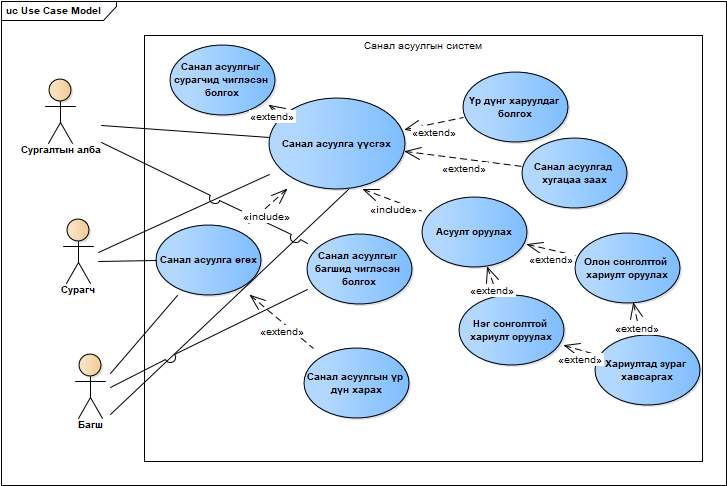
\includegraphics[scale=0.5]{usecase.png} 

\section{Class диаграмм}
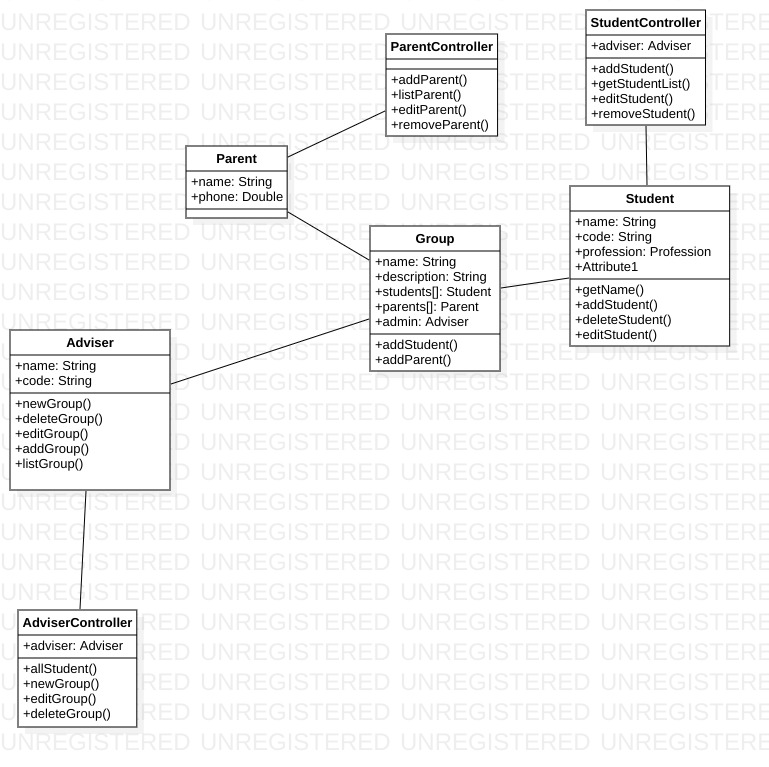
\includegraphics[scale=0.5]{ClassDiagram1.jpg} 


\section{Sequence диаграмм 1}
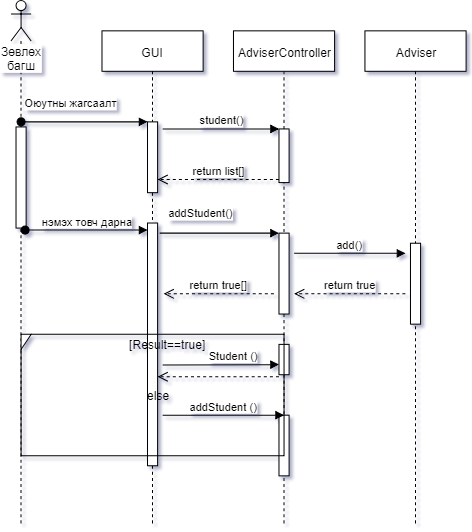
\includegraphics[scale=1]{Sequence1.png}
\section{Sequence диаграмм 2}
\section{Sequence диаграмм 3}

	\section{Бизнесс процессын диаграмм}
  
   	
   	\section{Activity диаграмм 1}
   	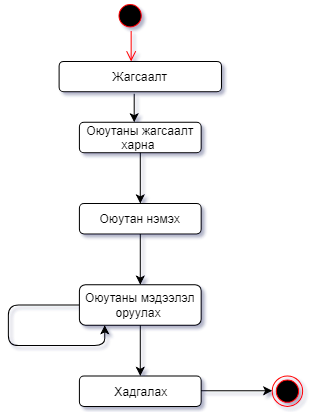
\includegraphics[scale=0.5]{Activity1.png} 
   	\section{Activity диаграмм 2}
   	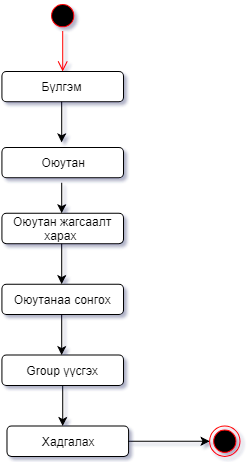
\includegraphics[scale=0.5]{Activity2.png} 
   	\section{Activity диаграмм 3}
   	
   	
   	\section{State диаграмм }
   	\section{Интерфейс зохиомж }
   	Дэлгэцийн зохиомж \\
   	
  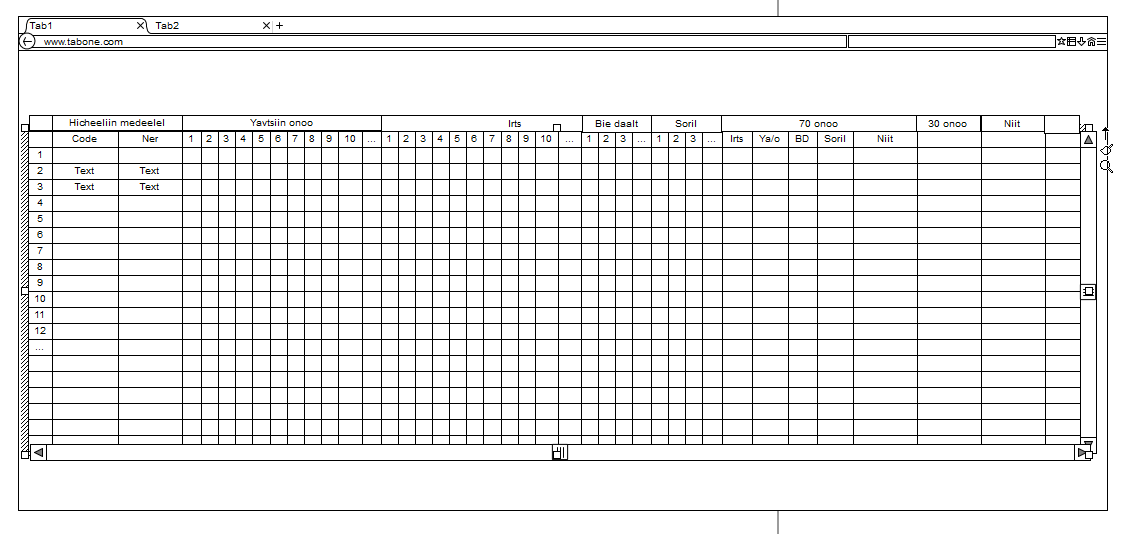
\includegraphics[scale=0.5]{delgets.png} 
   	
   	
   	
   	
\end{document}